\newcommand{\triangulationcomment}[1]{}


\begin{ccTexOnly}
\begin{center}
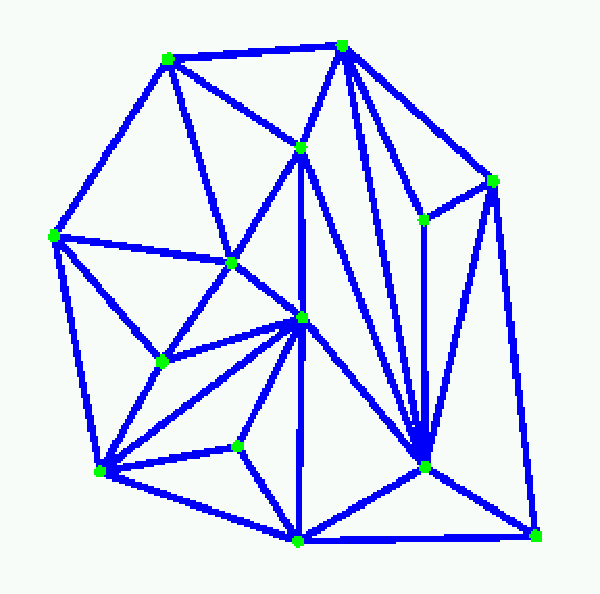
\includegraphics[width=6cm]{Triangulation_2/tr1} \hspace*{1cm} 
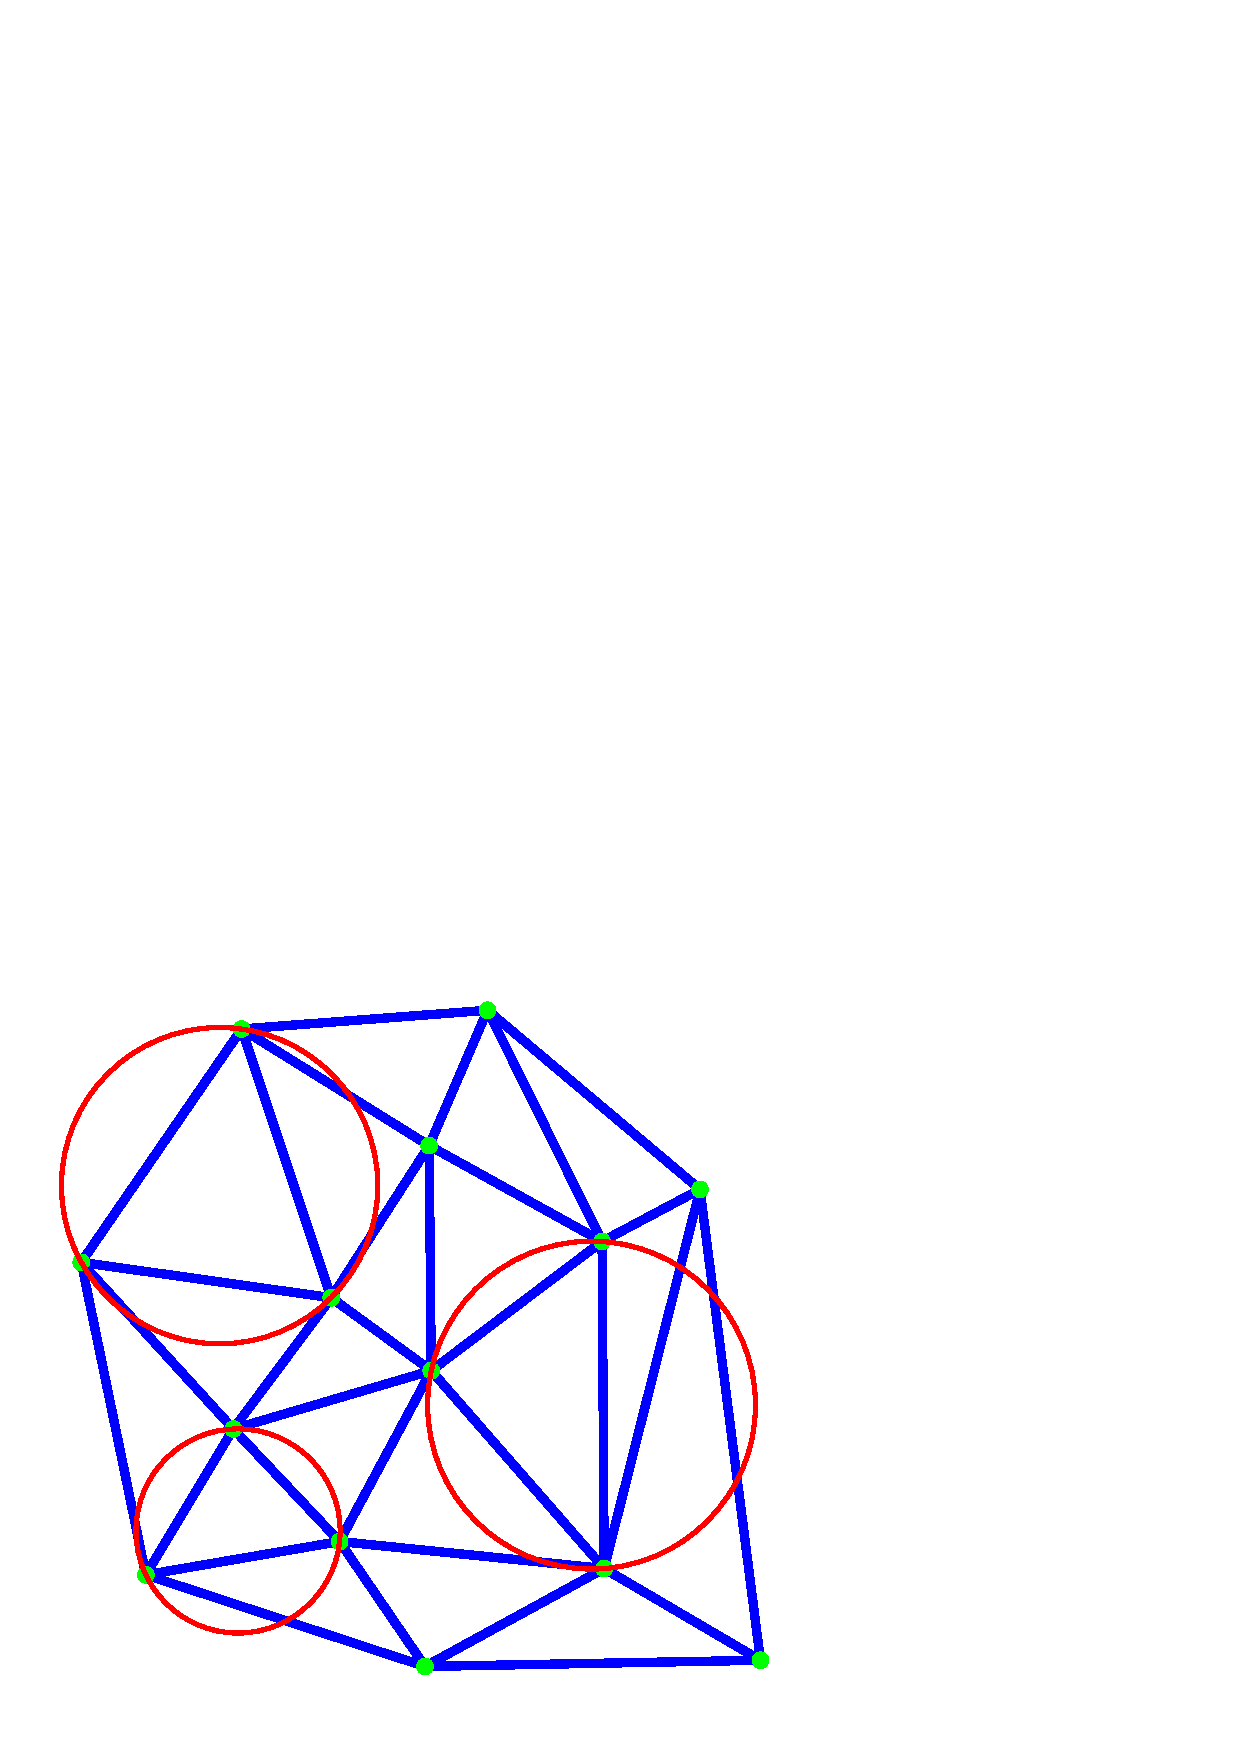
\includegraphics[width=6cm]{Triangulation_2/dt1} 
\end{center}
\end{ccTexOnly}
\begin{ccHtmlOnly}
<CENTER>
<img border=0 src="./tr1.gif" width=300>
<img border=0 src="./dt1.gif" width=300>
</CENTER>
\end{ccHtmlOnly}

This chapter describes the two dimensional triangulations
of \cgal. 
Section~\ref{Section_2D_Triangulations_Definitions} recalls the
main definitions about triangulations.
Sections~\ref{Section_2D_Triangulations_Representation} discusses
the way two-dimensional triangulations are represented in \cgal\ .
Section~\ref{Section_2D_Triangulations_Software_Design} presents
the overall software
design of the 2D triangulations package. 
The next sections present the different two dimensional triangulations classes
available in  \cgal\ : 
basic triangulations (section~\ref{Section_2D_Triangulations_Basic}),
Delaunay triangulations
(Section~\ref{Section_2D_Triangulations_Delaunay}),
regular triangulations
(Section~\ref{Section_2D_Triangulations_Regular}),
constrained triangulations
(Section~\ref{Section_2D_Triangulations_Constrained}),
and constrained Delaunay triangulations
(Section~\ref{Section_2D_Triangulations_Constrained_Delaunay}).
Section~\ref{Section_2D_Triangulations_Constrained_Plus}
describes a class which implements a constrained or
constrained Delaunay triangulation  with
an additional data structure 
to describe how the constraints are refined 
by the edges of the triangulations.
Section~\ref{Section_2D_Triangulations_Hierarchy}
describes a hierarchical data structure for
fast point location queries.
At last, Section~\ref{Section_2D_Triangulations_Flexibility} 
explains how the user can  benefit  from the flexibility 
of  \cgal\ triangulations using customized classes for faces
and vertices.

\section{Definitions\label{Section_2D_Triangulations_Definitions}}

A two dimensional triangulation can be roughly described as a set $T$
of triangular facets such that~:\\
- two facets either are  disjoint or share a lower dimensional
face (edge or vertex).\\
- the set of facets in  $T$ is connected for the adjacency relation. \\
- the  domain $U_T$  which is the union
of facets in $T$ has no singularity.


More precisely, a triangulation can be described 
as a simplicial complex.
Let us first record a few definitions.

A simplicial complex is a set $T$  of simplices such that~\\
- any face of a simplex in $T$ is a simplex in $T$ \\
- two simplices in $T$  either are disjoint or  share
  a common subface.

The dimension $d$ of a  simplicial complex is the 
maximal dimension of its simplices. \\
A simplicial complex $T$ is pure if any simplex of $T$
is included in a simplex of $T$ with maximal dimension. \\
Two simplexes in $T$ with maximal dimension $d$ are said to be
adjacent if they share a $(d-1)$ dimensional subface.
A simplicial complex is connected if the adjacency relation
defines a connected graph 
over  the set of simplices of $T$ with maximal dimension. \\
The union $U_T$ of all simplices in $T$ is called the domain of $T$.
A point $p$ in the domain of $T$ is said to singular 
if its surrounding in $U_T$
is neither a topological ball nor a topological disc.

Then, a two dimensional triangulation can be described as a 
two dimensional simplicial complex  that is pure,
connected and without singularity.

Each facet of a triangulation can be given an orientation
which in turn induces an orientation
on the edges incident to that facet. The orientation of two adjacent
facets are said to be consistent if they induce
opposite orientations on their common incident edge.
A triangulation is said to be orientable if 
the orientation of each facet can be chosen in such a way
that all pairs of incident facets have consistent orientations. 

The data stucture underlying \cgal\ triangulations
allows to represent the combinatorics of 
any  orientable two dimensional  triangulations
without boundaries. 
On top of this data structure, the 2D triangulations classes
take care of the geometric embedding  of the triangulation
and are designed to handle planar triangulations.
The plane of the tiangulation may be embedded in a higher
dimensional space.

The  triangulations of  \cgal\ are complete triangulations
which means  that their domain is  the
convex hull of  their vertices.
Because any planar triangulation
can be completed, this is not a real restriction.
For instance, a triangulation of a  polygonal region can be
constructed  and represented as a subset  of a constrained triangulation 
in which  the region boundary edges have been input as 
constrained edges (see
Section~\ref{Section_2D_Triangulations_Constrained},
\ref{Section_2D_Triangulations_Constrained_Delaunay} and 
\ref{Section_2D_Triangulations_Constrained_Plus}).

Strictly speaking, the term {\em face} should be used
to design  a face of any dimension,
and the two-dimensional faces of a triangulation 
should be properly called {\em facets}.
However, following a common usage, we hereafter often call {\em
faces}, the facets
of a two dimensional triangulation.

\section{Representation\label{Section_2D_Triangulations_Representation}}

\subsubsection{The set of faces}

A 2D triangulation  of \cgal\ can be viewed as a planar partition 
whose bounded faces are triangular and cover
the convex hull of the set of vertices. 
The single unbounded face of this partition
is the complementary of the convex hull. 
In many applications, such as Kirkpatrick's hierarchy
or incremental Delaunay construction, it is convenient to
deal with only triangular faces. Therefore, 
a fictitious vertex, called the \ccc{infinite vertex}
is added to the triangulation as well as
\ccc{infinite edges} and \ccc{infinite faces} incident to it..
Each infinite edge
is incident to the infinite vertex and to a vertex of the convex hull.
Each infinite face is incident to the infinite vertex
and to a convex hull edge. 

Therefore, each edge of the triangulation
is incident to exactly two faces
and the set of faces of a triangulation is topologically
equivalent to a two-dimensional sphere.
This extends to  lower dimensional triangulations
arising in degenerate cases or when the triangulations
as less than three vertices.
Including the infinite faces, 
a one dimensional triangulation
is a ring of edges and vertices
topologically equivalent to a $1$-sphere.
A zero dimensional triangulation, whose domain is reduced to a
single point, is represented by  two vertices that is
topologically equivalent to a $0$-sphere.

Note that
the \ccc{infinite vertex} has no significant
coordinates and that no geometric predicate can be applied on it
nor on an infinite face.

\begin{figure}
\begin{ccTexOnly}
\begin{center}
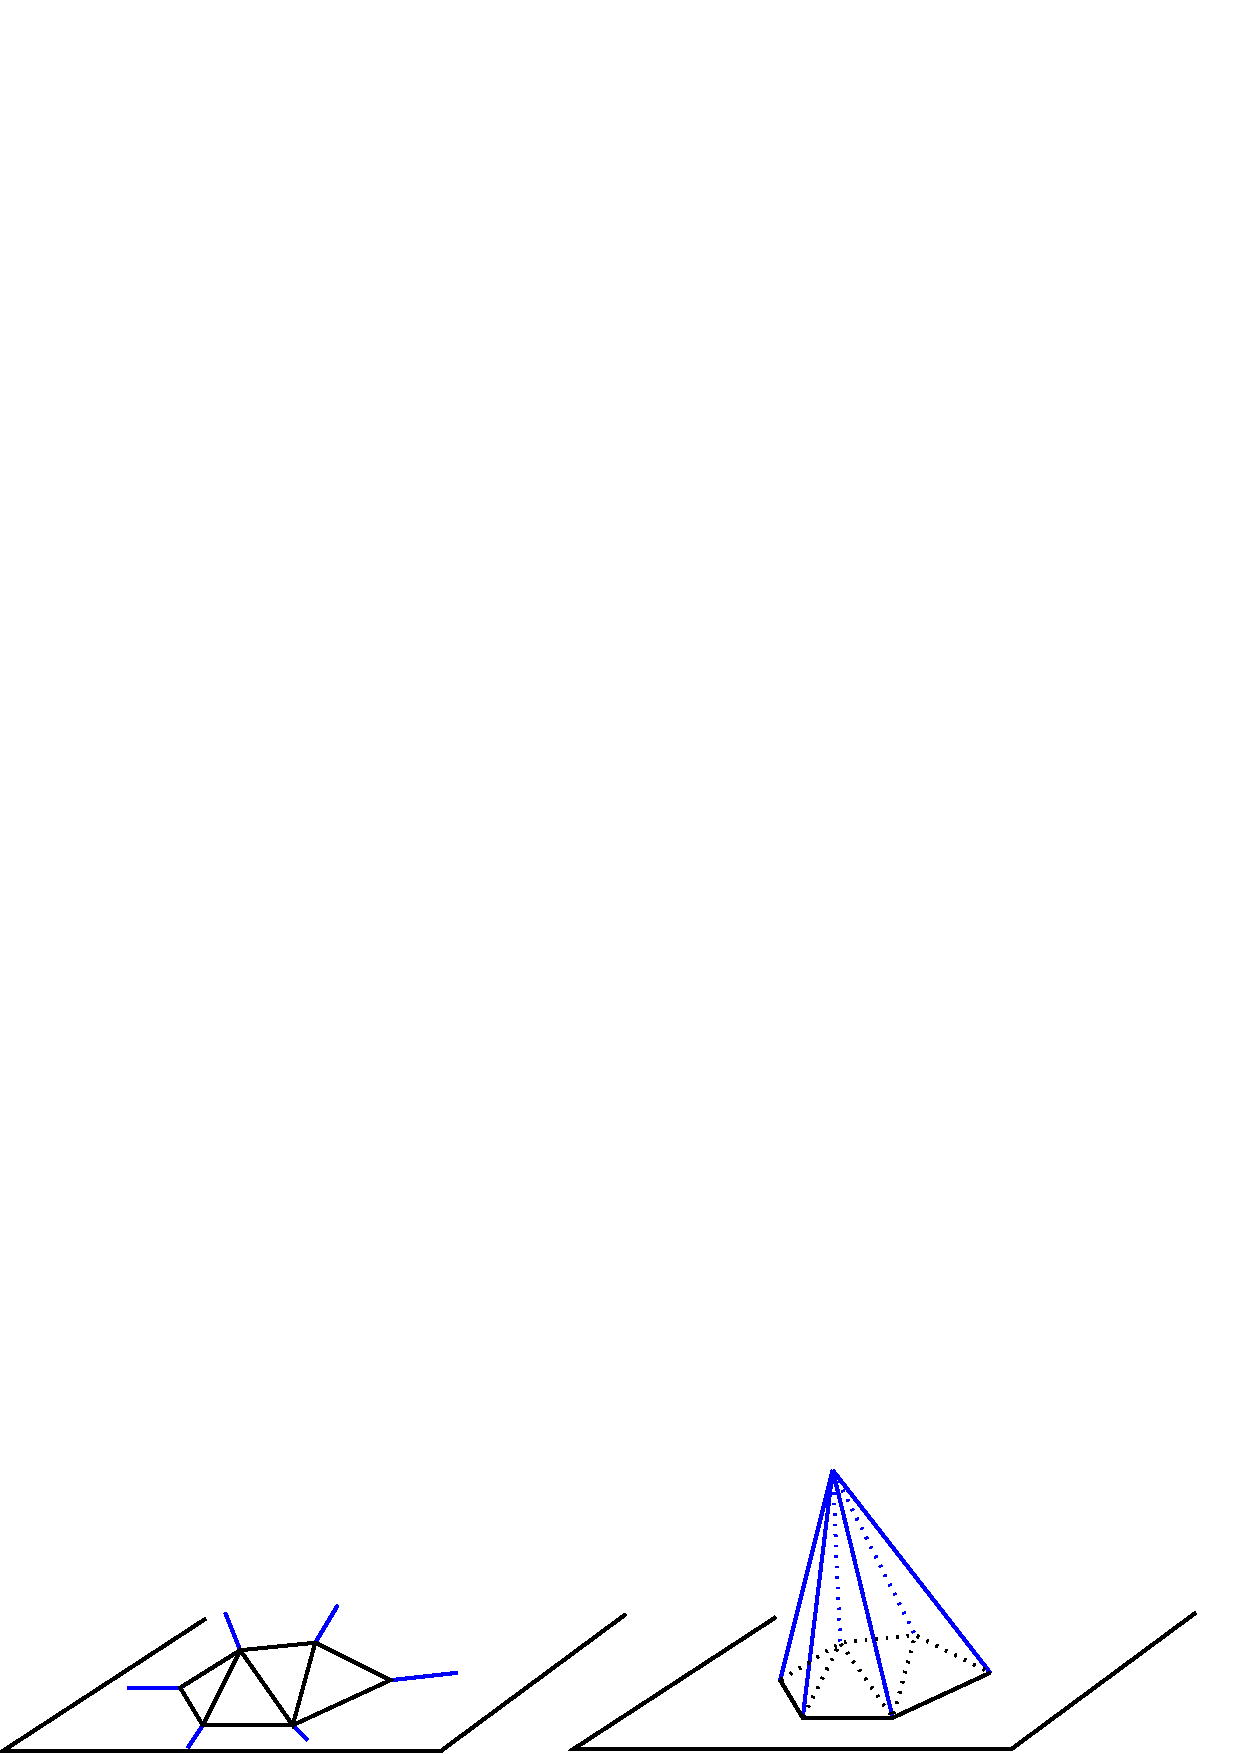
\includegraphics{Triangulation_2/infinite} 
\end{center}
\end{ccTexOnly}

\begin{ccHtmlOnly}
<CENTER>
<img border=0 src="./infinite.gif" align=center alt="Vertices at
infinity">
</CENTER>
\end{ccHtmlOnly}

\caption{Infinite vertex and infinite faces
\label{2D_Triangulation_Fig_infinite_vertex}}

\end{figure}




\subsubsection{ A representation based on faces and vertices}
Because a triangulation is  a set of
triangular faces with constant-size complexity,
triangulations are not implemented
as a layer on top of a planar map.
\cgal\ uses a proper internal
representation of triangulations based on faces and vertices
rather than on edges. Such a  representation
saves storage space and results in faster
algorithms~ \cite{bdty-tcgal-00}.

The basic elements of the representation are vertices and faces.
Each triangular face gives access to its three incident vertices 
and to its three adjacent faces. 
Each vertex gives access to one of its incident faces
and through that face to the circular list of its incident faces.

The three vertices of a face are indexed with 0, 1 and 2
in counterclockwise order. The neighbors of a face are also 
indexed with 0,1,2 in such a way that the neighbor indexed by \ccc{i}
is opposite to the vertex with the same index.
See Figure~\ref{2D_Triangulation_Fig_neighbors1}, 
 the functions \ccc{ccw(i)}
and \ccc{cw(i)} shown  on this figure
compute respectively $i+1$ and $i-1$ modulo 3.

The edges are not explicitly represented, they are only implicitely
represented through the adjacency relations of two faces.
Each edge has two implicit representations : the edge
of a face \ccc{f}  which is opposed to the vertex indexed \ccc{i},
can be represented as well as an edge of the \ccc{neighbor(i)} of 
\ccc{f}. 


 \begin{figure}
\begin{ccTexOnly}
    \begin{center}
     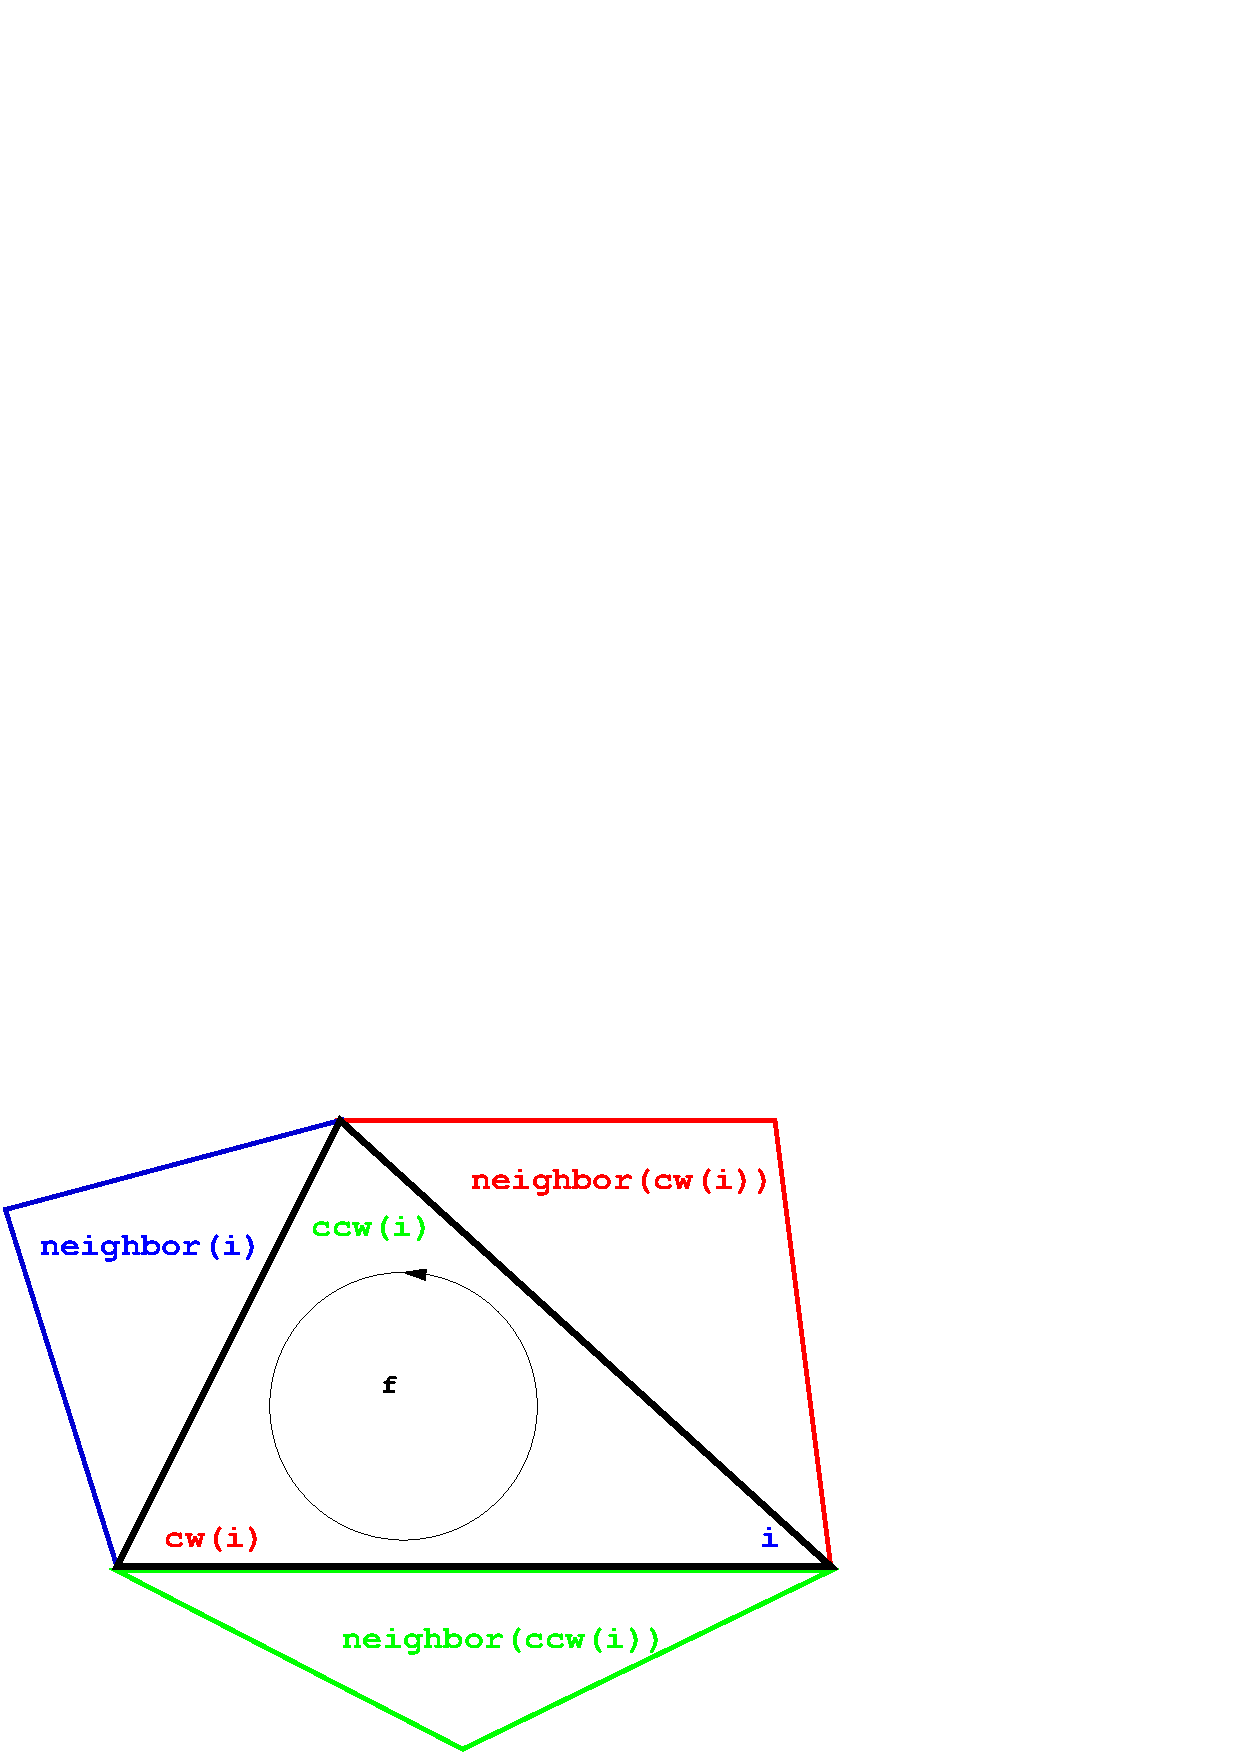
\includegraphics[width=6cm]{Triangulation_2/rep_bis} 
    \end{center}
\end{ccTexOnly} 
  \begin{ccHtmlOnly}
<CENTER>
<img border=0  src="./rep_bis.gif" width=400 align=center alt="Neighbors">
</CENTER>
\end{ccHtmlOnly} 

    \caption{Vertices and neighbors. 
    \label{2D_Triangulation_Fig_neighbors1} }
\end{figure}


\section{Software Design\label{Section_2D_Triangulations_Software_Design}}

The triangulations  classes of \cgal\  
provide high-level geometric functionalities
such as location of a point in the triangulation, insertion
or removal of a point.
They are build as a layer on top of a data structure
called the triangulation data structure.
The triangulation data structure   can be thought 
of as a container for the faces and vertices of the triangulation.
This data structure  also takes care
of all the combinatorial aspects of the triangulation.

This separation between the
geometric aspect and the combinatorial part
is reflected in the software design by the fact
that the triangulation classes have two template parameters :

\begin{itemize}
\item {} the first parameter stands for a
\textbf{geometric traits} class providing 
the geometric primitives (points, segments and triangles) 
of  the triangulation and the elementary
operations (predicate or constructions) on those objects.

\item {} the second parameter stands for a
\textbf{triangulation data structure} class. The concept
of triangulation data structure is described in
 Section~\ref{2D_TDS_Concept} of
Chapter~\ref{user_chapter_2D_Triangulation_Data_Structure}.
The triangulation data structure defines the types
used to represent the faces and vertices of the triangulation,
as well as additional types (handles, iterators and circulators)
to access and visit the faces and vertices.

\cgal\ provides the class \ccc{Triangulation_data_structure_2<Vb,Fb>}
as a  default model of triangulation data structure.
The class \ccc{Triangulation_data_structure_2<Vb,Fb>}
has two template parameters standing for
a vertex class and a face class.
\cgal\ defines concepts 
for these template parameters
and provide default models for these concepts.
The vertex and base classes are templated by the geometric
traits which allows them to have some knowledge of the geometric
primitives of the triangulation. 
Those default vertex and  face base classes
can be replaced by 
user customized base classes in order, for example, to deal
with additional properties attached to the vertices or faces
of a triangulation. See section~\ref{Section_2D_Triangulations_Flexibility}
for more details on the way to make use of this flexibility.
\end{itemize}

The Figure~\ref{2D_Triangulation_Fig_three_levels} summarizes the design of the
triangulation package, showing the  three layers
(base classes, triangulation data structure and triangulation)
forming this design.

\begin{figure}
\begin{ccTexOnly}
\begin{center}
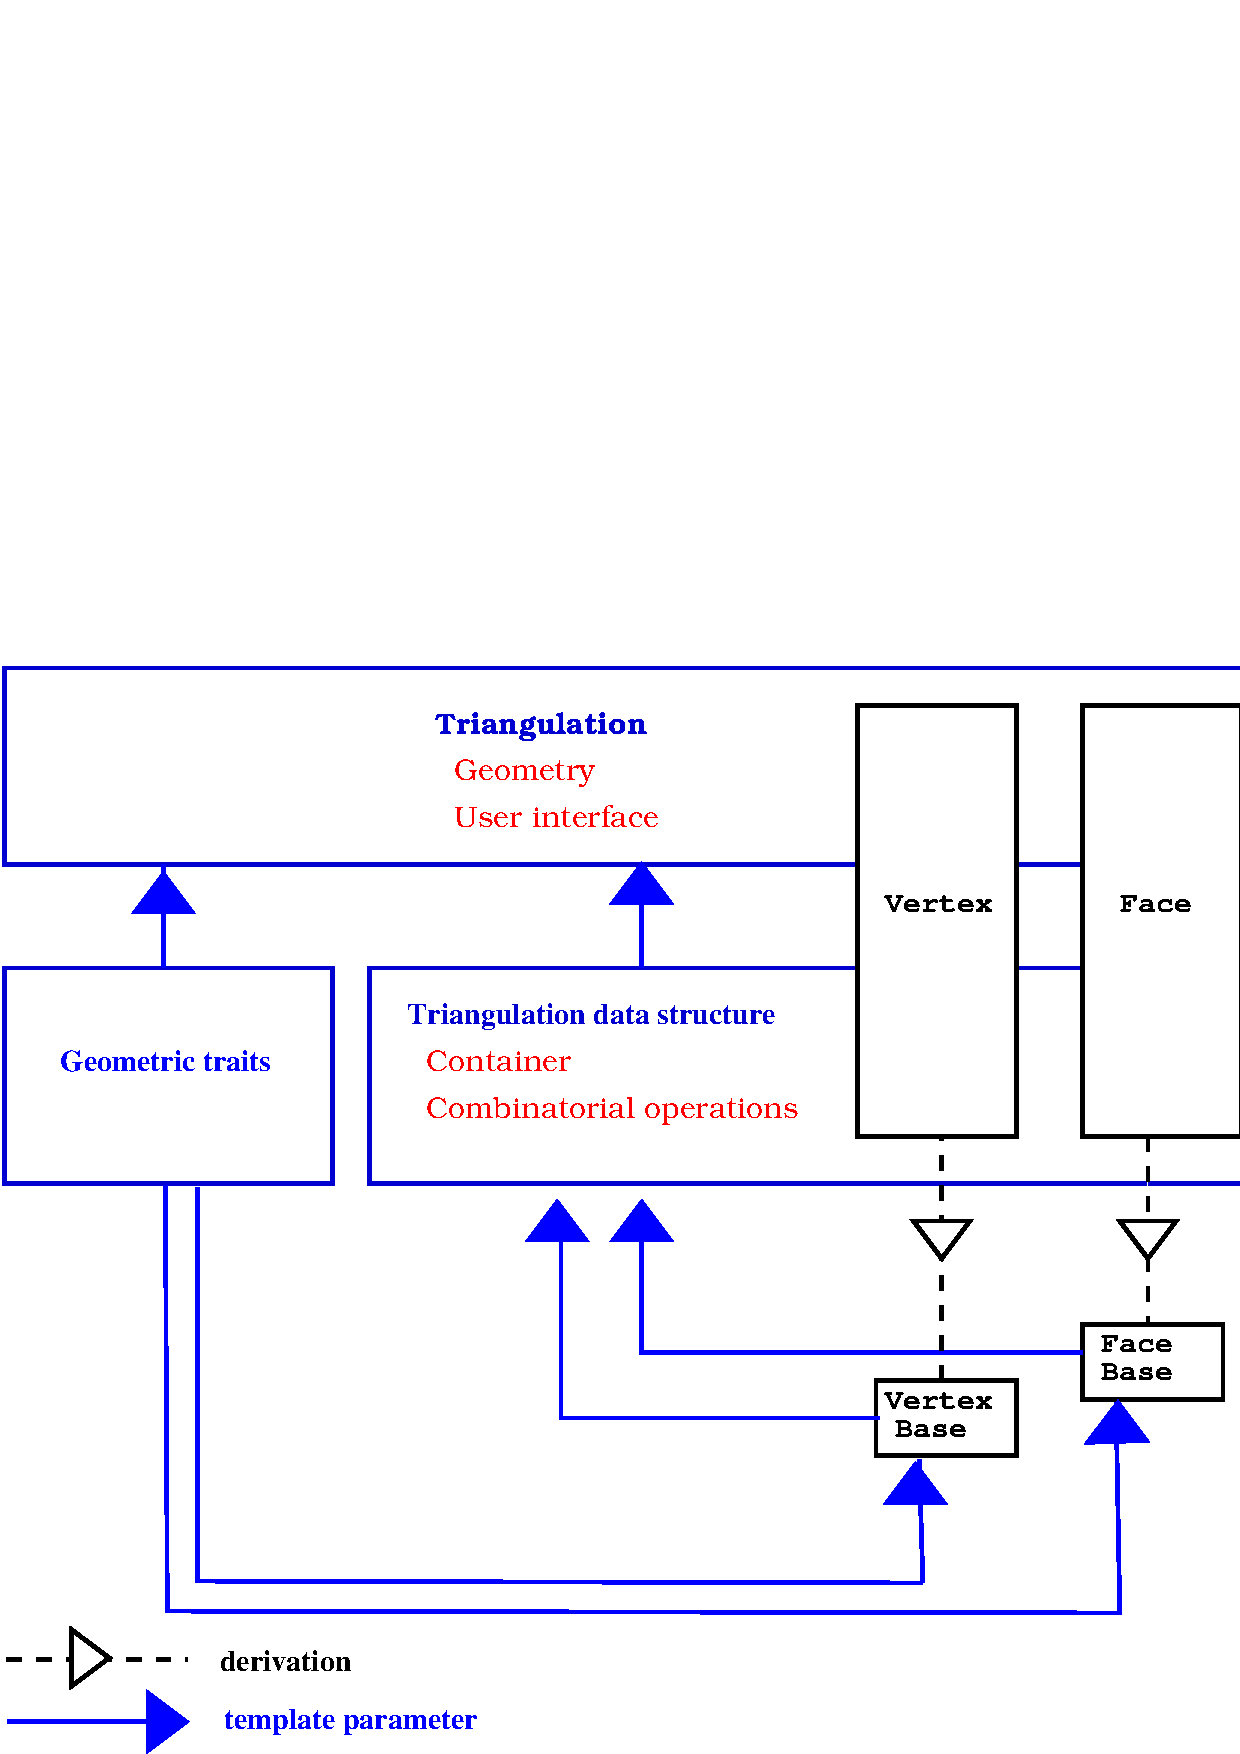
\includegraphics[width=13cm]{Triangulation_2/threelevels}
\end{center}
\end{ccTexOnly}

\begin{ccHtmlOnly}
<CENTER>
<br>
<img border=0 src="./threelevels.gif"  align=center alt="Three_levels">
</CENTER>
\end{ccHtmlOnly}

\caption{The triangulations software design.
\label{2D_Triangulation_Fig_three_levels}}
\end{figure}

The top triangulation  level, responsible for the geometric 
embedding of the  triangulation comes in different flavors 
according to the different kind of triangulations:
basic, Delaunay, regular, constrained or constrained Delaunay.
Each kind of triangulations correspond to a different
class. 
Figure~\ref{2D_Triangulation_Fig_derivation_tree}  summarizes the derivation dependencies
of \cgal\ 2D triangulations classes.
Any 2D triangulation class is parametrized by
a geometric traits and a triangulation data structure.
While a  unique concept \ccc{TriangulationDataStructure_2}
describes the   triangulation data structure requirements
for any  triangulation class, 
the concept of geometric traits actually depends
on the  triangulation class.
In general, the requirements for the vertex and face base classes 
are described by the basic concepts \ccc{TriangulationVertexBase_2}
and  \ccc{TriangulationFaceBase_2}. However, some  triangulation
classes requires base classes implementing
refinements 
of the basic concepts.


\begin{figure}
\begin{ccTexOnly}
\begin{center}
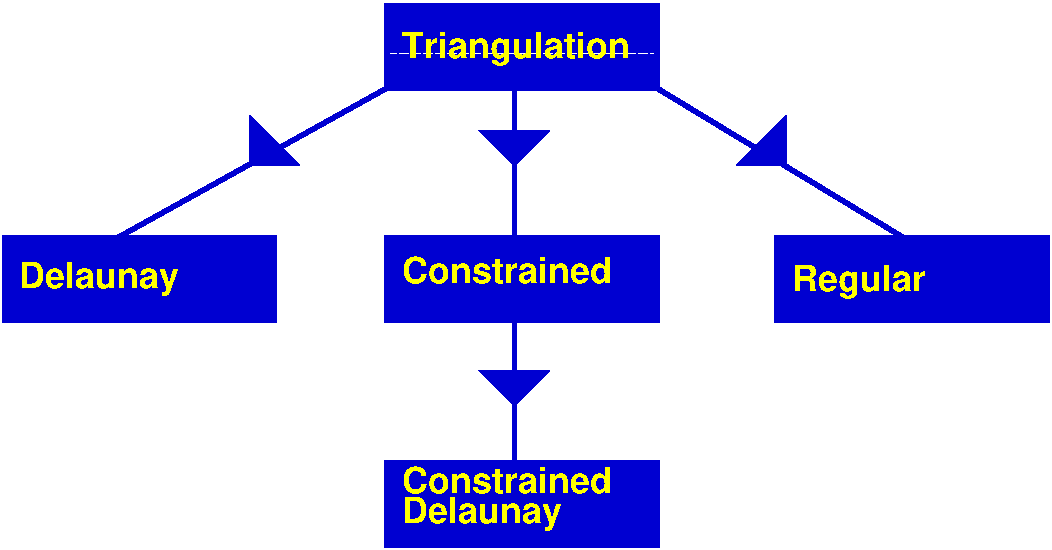
\includegraphics[width=13cm]{Triangulation_2/derivation_tree} 
\end{center}
\end{ccTexOnly}

\begin{ccHtmlOnly}
<br>
<CENTER>
<img border=0 src="./derivation_tree.gif" align=center>
</CENTER>
\end{ccHtmlOnly}

\caption{The derivation tree of 2D triangulations.}
\label{2D_Triangulation_Fig_derivation_tree}
\end{figure}

\section{Basic Triangulations\label{Section_2D_Triangulations_Basic}}

\subsection{Description\label{Subsection_2D_Triangulations_Basic_Description}}

The class \ccc{Triangulation_2<Traits,Tds>}
serves as a base class for the other
2D triangulations classes
and 
 implements the user
interface to a triangulation.




The vertices and faces of the triangulations are accessed through 
\ccc{handles},
\ccc{iterators} and \ccc{circulators}.
A handle is a model of the concept \ccc{Handle} which basically
offers the two dereference operators  \ccc{*}  and \ccc{->} .
A circulator is a type devoted to visit circular sequences.
Handles are used whenever the accessed element 
is not part of a sequence.
Iterators  and circulators are used
to visit  all or parts of the triangulation.


The iterators and circulators
are all bidirectional and non mutable.
The circulators and iterators are convertible to the 
handles with the same value type, so that 
when calling a member function,
any handle type argument can be replaced
by an iterator or a circulator
with the same value type.

The triangulation class allows to visit the vertices
and  neighbors of a face in clockwise or counterclockwise order. 

There are circulators  
to visit the edges or faces 
incident to a given vertex or the  vertices 
adjacent to it.
Another circulator type allows to visit all the faces
traversed by a given line.
Circulators step through infinite features as well as 
through finite ones. 

The triangulation class offers 
some iterators to visit all the 
faces, edges or vertices and also iterators to visit 
selectively the finite
faces, edges  or vertices.



The triangulation class provides methods to test
the infinite character of any feature,
and also methods to test the presence in the triangulation
of a particular feature (edge or face) given its vertices.

The triangulation class  provides a method to locate
a given point with respect to a triangulation.
In particular, this method reports wether the point
coincides with a vertex of the triangulation, lies on an edge,
in a face or outside of the convex hull. In case of a degenerate 
lower dimensional triangulation, the query point may also lie
outside the triangulation affine hull.

The triangulation class also provides
methods to locate a point with respect to
a given  finite face of the triangulation or with respect to its
circumcircle.
The faces of the triangulation and their circimcircles 
have the  counterclockwise orientation.

The triangulation can be modified by several functions~:
insertion of a point, removal of a vertex,
flipping  of an edge. The flipping of an edge
is possible when the union of the two incident faces
forms  a convex quadrilateral (see Figure~\ref{2D_Triangulation_fig_flip_bis}). 

\begin{figure}
\begin{ccTexOnly}
\begin{center}

\includegraphics{Triangulation_2/flip}
\end{center}
\end{ccTexOnly} 
\caption{Flip. \label{2D_Triangulation_fig_flip_bis}}
\begin{ccHtmlOnly}
<CENTER>
<img border=0 src="./Flip.gif" align=center alt="Flip">
</CENTER>
\end{ccHtmlOnly} 

\caption{Flip. \label{2D_Triangulation_fig_flip_bis}}
\end{figure}


\subsubsection{Implementation}

Locate is implemented by a line walk. The walk
begins  at  a vertex of the face which
is given
as an optional argument  or at an arbitrary vertex of the triangulation
 if no optional argument is given. It takes
time \ccTexHtml{$O(n)$}{O(n)} in the worst case, but only \ccTexHtml{$O(\sqrt{n})$}{O(sqrt(n))}
on average if the vertices are distributed uniformly at random.
The class \ccc{Triangulation_hierarchy_2<Traits,Tds>},
described in section~\ref{Section_2D_Triangulations_Hierarchy}, 
implements a data structure  designed to
offer an alternate  more efficient point location algorithm.

Insertion of a point is done by locating a face that contains the
point, and splitting this face into three new faces.
If the point falls outside the convex hull, the triangulation
 is restored by flips.  Apart from the location, insertion takes a
time \ccTexHtml{$O(1)$}{O(1)}. This bound is only an amortized bound
for points located outside the convex hull.

Removal of a vertex is done by removing all adjacent triangles, and
retriangulating the hole. Removal takes a time  at most proportionnal to
\ccTexHtml{$d^2$}{d^2}, where
 \ccTexHtml{$d$}{d} is the degree of the removed vertex,
which is \ccTexHtml{$O(1)$}{O(1)} for a random vertex.

The face, edge, and vertex iterators on finite features
are derived from their counterparts visiting all (finite and infinite)
features which are themselves derived from the corresponding iterators
of the triangulation data structure.


\subsubsection{Geometric Traits\label{Subsubsection_2D_Triangulation_Basic_Geometric_Traits}}

The geometric traits of a triangulation 
 is required to provide
the geometric objects (points, segments and triangles)
building up the triangulation
together with the geometric predicates on those objects.
The required predicates are: \\
- comparison of the \ccc{x} or \ccc{y} coordinates of two points.\\
- the orientation test which computes 
  the order type of three given point.

The concept
\ccc{TriangulationTraits_2}  describes the requirements for the 
geometric traits class of a triangulation.
 The \cgal\  kernel classes 
are models for  this  concept.
The \cgal\  library also provides dedicated models
of \ccc{TriangulationTraits_2} 
using the kernel geometric objects and predicates.
These classes are themselves templated with a \cgal\  kernel
and extract the required types and predicates from the kernel.
The traits class \ccc{Triangulation_euclidean_traits_2<R>}
is designed to deal with ordinary  two dimensional points.
The class \ccc{Triangulation_euclidean_traits_xy_3<R>} 
is a geometric traits class to build the triangulation
of a terrain. Such a triangulation is a two-dimensional
triangulation embedded  in  three dimensional space.
The data points are three-dimensional points.
The triangulation is 
build according to  the projections of those points
on the $xy$ plane  and then lifted up to the original
three-dimensional data points.
This is especially usefull
to deal with GIS terrains.
Instead of really projecting the  three-dimensional points and
maintaining a mapping between each point and its projection
 (which costs space and is error prone),
the traits class  supplies geometric predicates that ignore the
\ccc{z}-coordinates of the points.
See Section~\ref{Section_2D_Triangulations_Delaunay} for an example.
\cgal\ provides also the geometric traits classes
\ccc{Triangulation_euclidean_traits_yz_3<R>} and
\ccc{Triangulation_euclidean_traits_zx_3<R>} to
deal with projections on the
 \ccc{xz} plane  and  \ccc{yz}-plane,
respectively.

\subsection{Example of a Basic Triangulation\label{Subsection_2D_Triangulations_Basic_Example}}

The following program  creates a  triangulation of 2D points
using the  default kernel 
\ccc{Exact_predicate_inexact_constructions_kernel}
as geometric traits and the default triangulation data structure.
 The input points are read from a file 
and inserted in the triangulation.
Finally points on the convex hull are written to {\tt cout}. 
\ccIncludeExampleCode{Triangulation_2/triangulation_prog1.C}


\section{Delaunay Triangulations\label{Section_2D_Triangulations_Delaunay}}

\subsection{Description\label{Subsection_2D_Triangulations_Delaunay_Description}}
The class \ccc{Delaunay_triangulation_2<Traits,Tds>} is designed to represent
the Delaunay triangulation of a set of data points in the plane.
A  Delaunay triangulation
fulfills
the following {\em empty circle property} 
(also called {\em Delaunay property}): the circumscribing
circle of any facet of the triangulation 
contains no data point in its interior.
For a point set with no subset of four cocircular points
the Delaunay triangulation is unique, it is  dual
to the Voronoi diagram of the set of points.

The class \ccc{Delaunay_triangulation_2<Traits,Tds>} derives
from the class \ccc{Triangulation_2<Traits,Tds>}.

The class \ccc{Delaunay_triangulation_2<Traits,Tds>}
inherits the types defined by the 
basic class \ccc{Triangulation_2<Traits,Tds>}.
Additional types, provided by the traits class,
are defined to represent the dual Voronoi diagram.


The class \ccc{Delaunay_triangulation_2<Traits,Tds>}
overwrites the member functions that insert a new point
in the triangulation 
or remove a vertex  from it
to maintain the Delaunay property.
It also has a member function (\ccc{Vertex_handle
        nearest_vertex(const Point& p)})
to answer nearest neighbor queries
and member functions to construct the elements (vertices and edges)
of the dual Voronoi diagram.

\ccHeading{Geometric traits}
The geometric traits has to be a model of the concept
\ccc{DelaunayTriangulationTraits_2}
which refines the concept \ccc{TriangulationTraits_2}.
In particular this concept provides
the \ccc{side_of_oriented_circle} predicate
which, given four points \ccc{p,q,r,s}
 decides the position of  the point $s$  with respect to the circle
passing through $p$, $q$ and $r$. 
The \ccc{side_of_oriented_circle}
predicate actually defines the Delaunay triangulation.
Changing this predicate 
allows to build variant of Delaunay triangulations for different metrics
such that $L_1$ or $L_{\infty}$ metric or any metric defined by a
convex object. However, the user of an exotic metric
must be careful that the constructed triangulation 
has to be a triangulation of the convex hull
which means that convex hull edges have to be Delaunay edges.
This is granted for any smooth convex metric (like $L_2$)
and can be ensured for other metrics (like  $L_{\infty}$)
by the addition to the point set of well chosen sentinel points.

The \cgal\  kernel classes 
 and the class \ccc{Triangulation_euclidean_traits_2<R>}
are models of the concept \ccc{DelaunayTriangulationTraits_2}
for the euclidean metric.
The traits class for terrains,
\ccc{Triangulation_euclidean_traits_xy_3<R>},\\
\ccc{Triangulation_euclidean_traits_yz_3<R>}, and\\
\ccc{Triangulation_euclidean_traits_zx_3<R>} \\
are also models of  \ccc{DelaunayTriangulationTraits_2}
excapt that they do not fulfills 
the requirements for the duality functions and nearest vertex
queries.

\ccHeading{Implementation}
The insertion of a new point in the Delaunay triangulation
is performed using first the insertion member function
of the basic triangulation and second 
performing a sequence of flips to restore the Delaunay property. 
The number of flips that have to be performed is \ccTexHtml{$O(d)$}{O(d)}
if the new vertex has degree \ccTexHtml{$d$}{d} in the updated
Delaunay triangulation. For
points distributed uniformly at random, 
each insertion takes time \ccTexHtml{$O(1)$}{O(1)} on
average, once the point has been located in the triangulation.

Removal calls the removal in the triangulation and then retriangulates
the hole created in such a way that  the Delaunay criterion is
satisfied. Removal of a
vertex of degree \ccTexHtml{$d$}{d} takes time \ccTexHtml{$O(d^2)$}{O(d^2)}.
The degree $d$ is \ccTexHtml{$O(1)$}{O(1)} for a random
vertex in the triangulation.

After having performed a  point location, the
nearest neighbor of a point is found in time \ccTexHtml{$O(n)$}{O(n)} in the
worst case, but in time \ccTexHtml{$O(1)$}{O(1)}
for vertices distributed uniformly at random  and any query point. 


\subsection{Example : a Delaunay Terrain\label{Subsection_2D_Triangulations_Delaunay_Terrain}}

The following code  creates a Delaunay triangulation with 
the usual Euclidean metric for the vertical projection of a 
terrain model. The points have elevation, that is they are 3D points,
but the predicates used to build the  Delaunay triangulation
are computed using only  the $x$ and $y$ coordinates  
of these points. 
\ccIncludeExampleCode{Triangulation_2/terrain.C}

\subsection{Example : Voronoi Diagram\label{Subsection_2D_Triangulations_Voronoi}}
\ccIndexMainItem{Voronoi diagram}
The following code computes the edges of Voronoi diagram
of a set of data points
and counts  the number of finite edges and the number of rays
of this diagram
\ccIncludeExampleCode{Triangulation_2/voronoi.C}


\section{Regular Triangulations\label{Section_2D_Triangulations_Regular}}

\subsection{Description\label{Subsection_2D_Triangulations_Regular_Description}}
\ccIndexMainItem{power diagram}
Let ${  PW} = \{(p_i, w_i), i = 1, \ldots , n \}$ be a set of 
weighted points where each $p_i$ is a point and each $w_i$
is a scalar called the weight of point $p_i$.
Alternatively, each weighted point $(p_i, w_i)$ can be regarded
as a sphere (or a circle, depending on the dimensionality
of $p_i$)  with center $p_i$ and radius $r_i=\sqrt{w_i}$.

The power diagram of the set ${  PW}$ is a space partition in which
 each cell corresponds to a sphere $(p_i, w_i)$ of ${  PW}$
and is the locus of points  $p$ whose power with respect to $(p_i, w_i)$
is less than its power with respect to any other sphere 
in ${  PW}$. In the two-dimensional space,
the dual of this diagram is a triangulation 
whose domain covers the convex hull of the set 
${  P}= \{ p_i, i = 1, \ldots , n \}$ of center points
and whose vertices form a subset of ${  P}$.
Such a triangulation is called a regular triangulation.
Three points $p_i, p_j$ and $p_k$ of ${  P}$
form a triangle in the regular triangulation of ${  PW}$
iff there is a point $p$ of the plane with equal 
powers with respect to $(p_i, w_i)$, $(p_j, w_j)$
and $(p_k, w_k)$ and such that this power 
is  less than the power of $p$
with respect to any other sphere in  ${  PW}$.

Let us defined the power product of two weighted points
$(p_i, w_i)$ and $(p_j, w_j)$ as:
\[\Pi(p_i, w_i,p_j, w_j) = p_ip_j ^2 - w_i  - w_j  .\]
$\Pi(p_i, w_i,p_j, 0)$ is simply the power of point $p_j$
with respect to the sphere $(p_i, w_i)$, and two weighted points 
are said to be orthogonal if their power product is null.
The power circle of three weighted points
 $(p_i, w_i)$, $(p_j, w_j)$
and $(p_k, w_k)$ is defined as the unique circle
$(\pi, \omega)$  orthogonal to
 $(p_i, w_i)$, $(p_j, w_j)$
and $(p_k, w_k)$.

The regular triangulation of the sets ${  PW}$
satisfies the following {\em regular property} (which just reduces to the 
Delaunay property when all the weights are null):
a triangle $p_ip_jp_k$ is a face of the regular triangulation
of ${  PW}$ iff the power product of any weighted point
 $(p_l, w_l)$ of ${  PW}$ with the power circle of
 $(p_i, w_i)$, $(p_j, w_j)$ and $(p_k, w_k)$ is positive or null.
We call  power test of  $(p_i, w_i)$, $(p_j, w_j)$, $(p_k, w_k)$,
and $(p_l, w_l)$,  the predicates which amount to compute
the sign of 
the power product of $(p_l, w_l)$ with respect to
the power circle of
 $(p_i, w_i)$, $(p_j, w_j)$ and $(p_k, w_k)$.
This predicate amounts to computing the sign of
the following
determinant
\[\left| \begin{array}{cccc}
1  &  x_i  &  y_i  &  x_i ^2 + y_i ^2 - w_i  \\
1  &  x_j  &  y_j  &  x_j ^2 + y_j ^2 - w_j  \\
1  &  x_k  &  y_k  &  x_k ^2 + y_k ^2 - w_k  \\
1  &  x_l  &  y_l  &  x_l ^2 + y_l ^2 - w_l
\end{array}
\right|
\]

A pair of neighboring faces $p_ip_jp_k$
and $p_ip_jp_l$ is said to be locally regular
(with respect to  the weights in ${  PW}$)
if the power test of $(p_i, w_i)$, $(p_j, w_j)$, $(p_k, w_k)$,
and $(p_l, w_l)$ is positive.
A classical  result of computational geometry
establishes that a triangulation of the convex hull of ${  P}$
such that any pair of neighboring faces is regular with respect
to ${  PW}$, is a
 regular triangulation of ${  PW}$.

Alternatively, the regular triangulation
of the weighted points set ${  PW}$
can be obtained as the projection
on the two dimensional plane of the convex hull of the set of three
dimensional points 
${  P'}= \{ (p_i,p_i ^2 - w_i ), i = 1, \ldots , n \}$.

The class \ccc{Regular_triangulation_2<Traits, Tds>}
 is designed to maintain the
regular triangulation of a set of $2d$ weighted points.
It derives from the class \ccc{Triangulation_2<Traits, Tds>}.
The functions \ccc{insert} and 
\ccc{remove} are overwritten to handle weighted points
and maintain the regular
property.
The vertices of the regular triangulation
of a set of weighted points ${PW}$ correspond  only to a subset
of ${PW}$.
Some of the input
weigthed points have no cell in the dual power diagrams
and therefore do not correspond to a vertex of the regular
triangulation.
Such a point is called a hidden point.
Because hidden points can reappear later on as vertices
when  some other point is removed,
they  have to be stored somewhere. 
The regular triangulation  store those points in special vertices, called
hidden vertices. 
A hidden point can reappear as vertex of the triangulation
only when the two dimensional face that hides it
is removed from the triangulation. To deal with this feature,
each face of a regular triangulation stores a list of hidden vertices.
The points in those vertices 
are reinserted in the triangulation  when the face
is removed.

Regular triangulation have member functions to construct
the vertices and edges of the dual power diagrams.

\subsubsection{The geometric traits}
The geometric traits of a regular triangulation
must provide a weighted point type
and a power test on these weighted points.
The concept 
\ccc{RegularTriangulationTraits_2},
is a refinement of the concept
\ccc{TriangulationTraits_2}. \cgal\ provides 
the class
\ccc{Regular_triangulation_euclidean_traits_2<Rep,Weight>}
which is a model for the traits concept
\ccc{RegularTriangulationTraits_2}.
The class \ccc{Regular_triangulation_euclidean_traits_2<Rep,Weight>}
derives  from the class
\ccc{Triangulation_euclidean_traits_2<Rep>}
and uses a \ccc{Weighted_point} type
derived from the type \ccc{Point_2} of
\ccc{Triangulation_euclidean_traits_2<Rep>}.

\textbf{Note that, since the type \ccc{Weighted_point} is not defined 
in \cgal\ kernels, plugging a filtered kernel  such as 
\ccc{Exact_predicates_exact_constructions_kernel} in
\ccc{Regular_triangulation_euclidean_traits_2<K,Weight>} will in fact
not provide exact predicates on  weighted points.}
To solve this, there is also another model of the traits concept,
\ccc{Regular_triangulation_filtered_traits_2<FK>}, which is providing filtered
predicates (exact and efficient). The argument \ccc{FK} must be a
model of the \ccc{Kernel} concept, and it is also restricted to be a
instance of the \ccc{Filtered_kernel} template. 



\subsubsection{The Vertex type and Face Type of a Regular Triangulation}

The base vertex type of a regular triangulation
includes a boolean to mark the hidden state of the vertex.
Therefore  CGAL defines the concept
\ccc{RegularTriangulationVertexBase_2} which refine
the concept \ccc{TriangulationVertexBase_2}
and provides a default model 
for this concept.

The base face type of a regular triangulation
is required to provide a list of hidden vertices,
designed to store the points hidden by the face. It has to be a model
of the concept \ccc{RegularTriangulationFaceBase_2}.
\cgal\ provides the templated class 
\ccc{Regular_triangulation_face_base_2<Traits>}
as a default base class for faces of regular triangulations.



\subsection{Example : a Regular Triangulation\label{Subsection_2D_Triangulations_Regular_Example}}

The following code  creates a regular triangulation 
of a set of weighted points and ouput the number
of vertices and the number of hidden vertices.

\ccIncludeExampleCode{Triangulation_2/regular.C}


\section{Constrained Triangulations\label{Section_2D_Triangulations_Constrained}}

%\subsection{Description}
\label{Subsection_2D_Triangulations_Constrained_Description}
A constrained triangulation is a triangulation of a set of points
that has to include among its edges 
a given set of segments joining the points. The corresponding 
edges are called {\em constrained edges}. 

The endpoints of constrained edges are of course vertices of the
triangulation. However the triangulation may include
include other vertices as well.
There are three versions of  constrained triangulations.
\begin{itemize}
\item
In the basic version, the constrained triangulation 
does not handle intersecting constraints, and the set of input 
constraints is required to be a set of segments that do not intersect
except possibly at their endpoints. Any number of constrained edges
are allowed to share the same endpoint.  Vertical constrained edges or
constrained edges with null length are allowed.
\item 
The two other versions support intersecting input constraints.
In those versions, input constraints are allowed to be
intersecting, overlapping or partially
overlapping segments.
The triangulation introduces  additional  vertices at each point that
is the proper intersection points of  two 
constraints. A single constraint intersecting other
constraints will then appear as several edges in the triangulation.
The two versions dealing with intersecting constraints differ
in the way intersecting constraints are dealt with.
\begin{itemize}
\item
 One of them is
designed to be robust when predicates are evaluated exactly but
constructions (i. e.  intersection computations) are
approximative.
\item
The other one is designed to be used 
with exact arithmetic (meaning exact
evaluation of predicates and exact computation of intersections.)
This last version finds its full efficiency  when used in conjunction
with a constraint hierarchy data structure (which allows one to avoid the
cascading of intersection computations)
as provided in the class
\ccc{Constrained_triangulation_plus_2}. See
section~\ref{Section_2D_Triangulations_Constrained_Plus}.
\end{itemize}
\end{itemize}


\begin{ccTexOnly}
\begin{center} 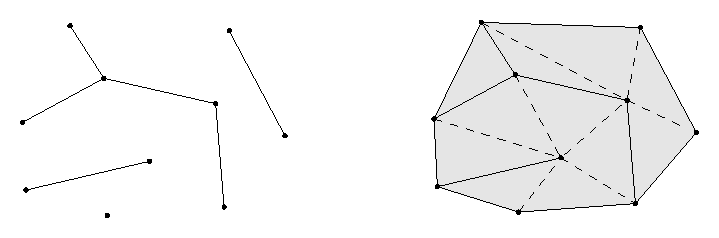
\includegraphics{Triangulation_2/constraints} \end{center}
\end{ccTexOnly}
 
\begin{ccHtmlOnly}
<CENTER>
<img border=0 src="./constraints.gif" align=center alt="A set of
constraints and its constrained triangulation">
</CENTER>
\end{ccHtmlOnly}

A constrained triangulation is represented in the CGAL library as an
object of the class \ccc{Constrained_triangulation_2<Traits,Tds,Itag>}.
The third parameter \ccc{Itag} is the intersection tag
which serves to choose how intersecting constraints
are dealt with. This parameter has to be instantiated
by one of the following classes~:
\ccc{CGAL::No_intersection_tag} when input constraints do not
intersect \\
\ccc{CGAL::Exact_predicates_tag} if the geometric traits provides
exact predicates but approximative constructions \\
\ccc{CGAL::Exact_intersections_tag} when an exact predicates
and exact constructions are provided.

The class \ccc{Constrained_triangulation_2<Traits,Tds, Itag>}
inherits from \ccc{Triangulation_2<Traits,Tds>}.
It defines an additional type \ccc{Constraint}
to represent the constraints. A
constraint is represented as a pair of points.

A  constrained triangulation can be created
from a
list of constrained edges.
The class \ccc{Constrained_triangulation_2<Traits,Tds,Itag>}
overrides the insertion and removal of a point to take care of the
information about constrained edges. The class also allows inline
insertion of a new constraint, given by its two endpoints
or the removal of a constraint.

\subsubsection{The Geometric Traits}
The geometric traits of a constraint triangulation
 has to be a model
of the concept \ccc{TriangulationTraits_2}.
When intersections of input constraints are supported, 
the geometric traits class has to be a model 
of the concept \ccc{ConstrainedTriangulationTraits_2}
which refines the concept \ccc{TriangulationTraits_2}
providing  additional function object types
to compute the intersection of two segments.

\subsubsection{The Base Face of a Constrained Triangulation}
 The information about constrained edges is stored in the 
faces of the triangulation. The base face of a Constrained Triangulation
has to be a model for the concept \ccc{ConstrainedTriangulationFaceBase_2}
which refines the concept \ccc{TriangulationFaceBase_2}.
The concept \ccc{ConstrainedTriangulationFaceBase_2}
requires  member functions
 the get and set the constrained status of the edges.

\cgal\ provides a default base face class
for constrained triangulations. This class, named
\ccc{Constrained_triangulation_face_base_2<Traits>},
derives from the class
\ccc{Triangulation_face_base_2<Traits>}
and adds three booleans to store the status of its edges. 

%\subsubsection{A Constrained Triangulation Class for Animation Purposes
%\cgal\ provides 
%a class  \ccc{Constrained_triangulation_demo_2<Traits,Tds>}
%specially designed to show an animation of the sweep algorithm 
%that builds a 
%constrained triangulation from a list of constraints.

\begin{figure}
\begin{ccTexOnly}
\begin{center}
\includegraphics[width=5cm]{Triangulation_2/poisson}
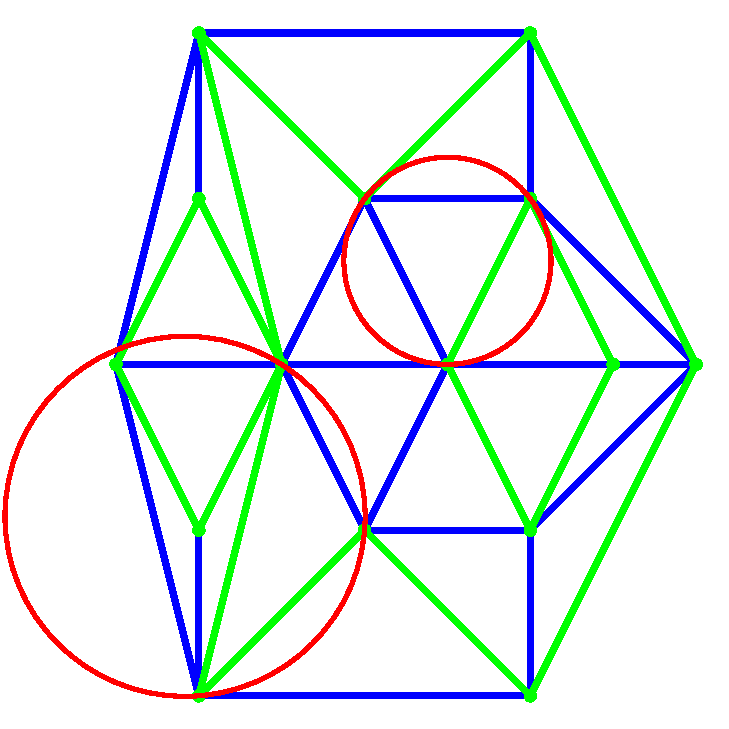
\includegraphics[width=5cm]{Triangulation_2/del_poisson}
\end{center}
\end{ccTexOnly}

\begin{ccHtmlOnly}
<CENTER>
<img border=0 src="./poisson.gif" width=300 alt=" Constrained triangulation">
<img border=0 src="./del_poisson.gif" width=300 alt="Constrained Delaunay triangulation">
</CENTER>
\end{ccHtmlOnly}

\caption{Constrained and Constrained Delaunay triangulation : 
 the constraining edges are the green edges,  a constrained
triangulation is shown on the left, the constrained Delaunay
triangulation with two examples of circumcircles is shown on the right.}
\label{2D_Triangulation_Fig_constrained}
\end{figure}


\section{Constrained Delaunay Triangulations\label{Section_2D_Triangulations_Constrained_Delaunay}}

%\subsection{Description}
\label{Subsection_2D_Triangulations_Constrained_Delaunay_Description}
A constrained Delaunay triangulation is a triangulation with
constrained edges which tries to be as much Delaunay as possible.
As constrained edges are not necessarily Delaunay edges,
the triangles of a constrained Delaunay triangulation do not
necessarily fulfill the empty circle property
but they fulfill a weaker \ccc{constrained empty circle property}.
 To state this property,
it is convenient to think of  constrained
edges as blocking the view. Then, a triangulation is 
constrained Delaunay iff
 the circumscribing circle
of any facet encloses 
no vertex  visible
from the interior of the facet.
As in the case of constrained triangulations, three different versions
of Delaunay constrained triangulations are provided. The first version
handle set of constraints which do not intersect except possibly
at the endpoints. The two other versions 
handle intersecting input constraints. One of them
 is designed to be designed to be robust
when used in conjunction with a geometric traits
providing exact predicates and approximative constructions
(such as a \ccc{CGAL::Filtered_Kernel} or any kernel providing
filtered exact predicates). The third version is designed to be used
with an exact arithmetic number type.




The \cgal\ class
\ccc{Constrained_Delaunay_triangulation_2<Traits,Tds,Itag>}
is designed to represent
constrained Delaunay triangulations.

As in the case of constraints triangulation, the third parameter 
\ccc{Itag} is the intersection tag
and serves to choose how intersecting constraints
are dealt with. It can be instantiated with one of the following
class~: \ccc{CGAL::No_intersection_tag},
\ccc{CGAL::Exact_predicates_tag},
\ccc{CGAL::Exact_intersections_tag} 
(see Section~\ref{Section_2D_Triangulations_Constrained}.

A constrained Delaunay triangulation is not a Delaunay
triangulation but it is a constrained triangulation.
Therefore the class
\ccc{Constrained_Delaunay_triangulation_2<Traits,Tds,Itag>}
derives from
the class \ccc{Constrained_triangulation_2<Traits,Tds,Itag>}.

The constrained Delaunay triangulation
has member functions to override the 
insertion and removal of a point or of a constraint.
Each of those member function takes care
to  restore
 the constrained empty circle
property.

\subsubsection{The Geometric Traits}
 The geometric traits 
of a constrained Delaunay triangulation is required
to provide the \ccc{side_of_oriented_circle} predicate as the geometric traits
of a Delaunay triangulation and has to a model of the concept
\ccc{DelaunayTriangulationTraits_2}. When intersecting input
constraints
are supported the geometric traits is further required 
to provide function objects to compute constraints intersections.
Then the geometric traits has to be at the same time a model
of the concept \ccc{ConstrainedTriangulationTraits_2}.



\subsubsection{The face base class}
Information about the status (constrained or not)
of the edges of the triangulation has to be stored
in the face class
 and the base face class
of a constrained Delaunay triangulation has to be a model
of \ccc{ConstrainedTriangulationFaceBase_2}.




\subsection{Example : a  constrained Delaunay triangulation\label{Subsection_2D_Triangulations_Constrained_Delaunay_Example}}
The following code inserts a set of intersecting constraint segments
into a triangulation 
and counts the number of constrained edges of the
resulting triangulation.

\ccIncludeExampleCode{Triangulation_2/constrained.C}


\section{Constrained Triangulations Plus\label{Section_2D_Triangulations_Constrained_Plus}}

The class \ccc{Constrained_triangulation_plus_2<Tr>}
provides a constrained triangulation with an additional data
structure called the  constraint hierarchy 
that keeps track of  the input constraints and of their refinement
in the triangulation.
The class \ccc{Constrained_triangulation_plus_2<Tr>}
inherits from its template parameter Tr, which has to be instantiated
by a constrained  or constrained Delaunay  triangulation.
According to its intersection tag, the base class
will support intersecting input constraints or not.
When intersections of input constraints are supported,
the base class constructs a triangulation  of the  arrangement
of the constraints,
introducing new vertices at each proper intersection
points and  refining the input constraints into subconstraints
which appear as  edges (more precisely as constrained edges) of the
triangulation.  The  data structure maintains for each 
input constraint
the sequence of intersection vertices added on this constraint.
The constraint hierarchy also allows the user to retrieve the set
of constrained edges of the triangulation, and for each
constrained edge,  the set of input constraints that overlap it.

The class \ccc{Constrained_triangulation_plus_2<Tr>}
is especially useful when the base constrained triangulation class
handles intersections of constraints and uses an exact number type,
i.e. when its intersection tag is \ccc{CGAL::Exact_intersections_tag}.
Indeed in this case, the \ccc{Constrained_triangulation_plus_2<Tr>}
is specially designed to avoid cascading in the computations of
intersection  points.

\subsection{Example : Building a triangulated arrangement of segments}

The following code inserts a set of intersecting constraint segments
into a triangulation 
and counts the number of constrained edges of the
resulting triangulation.


\ccIncludeExampleCode{Triangulation_2/constrained_plus.C}




\section{The Triangulation Hierarchy\label{Section_2D_Triangulations_Hierarchy}}


The class \ccc{Triangulation_hierarchy_2<Tr>}
implements a triangulation augmented with
a data structure to answer efficiently  point location queries.
The data structure is a hierarchy 
of triangulations. The triangulation at the lowest level is
the original triangulation where operations and point location are to 
be performed.
Then at each succedding level, the data structure
stores a triangulation of a small random sample of the vertices
of the triangulation at the preceeding level. Point location
is done through a top down nearest neighbor query.
The nearest neighbor query is first
performed naively in the top level triangulation.
Then, at each following level, the nearest neighbor at that level
is found through a linear walk performed from
the nearest neighbor found at the preceeding level.
Because the number of vertices in each triangulation is only a small
fraction of the number of vertices of the preceeding triangulation,
the data structure remains small and achieves fast point location 
queries  on real
data. As proved in~\cite{d-iirdt-98}, this structure has an optimal behaviour
when it is built for Delaunay triangulations.
However it can be used as well for other triangulations
and the class \ccc{Triangulation_hierarchy_2<Tr>} is templated by a parameter
which is to be instantiated by one of the \cgal\ triangulation
classes. 

The class \ccc{Triangulation_hierarchy_2<Tr>} inherits from the
triangulation type passed as template parameter \ccc{Tr}. 
The insert and remove member functions
are  overwritten to update the data structure at each operation.
The locate queries are also overwritten to take advantage of the data
structure for a fast processing.

\subsubsection{The Vertex of a Triangulation Hierarchy}
The base vertex class  of a triangulation hierarchy 
has to be a model of the
concept
\ccc{TriangulationHierarchyVertexBase_2} which extends
the concept \ccc{TriangulationVertexBase_2}.
This extension adds
access and setting member functions 
for two pointers  to the corresponding vertices in the 
triangulations of the next and preceeding levels.

\cgal\ provides the class \ccc{Triangulation_hierarchy_vertex_base_2<Vb>}
which is a model for the concept 
\ccc{TriangulationHierarchyVertexBase_2}.
This class is templated by a parameter \ccc{Vb}
which is to be instantiated by a model of  the concept
\ccc{TriangulationVertexBase_2}.
The class \ccc{Triangulation_hierarchy_vertex_base_2<Vb>} inherits
from its template parameter \ccc{Vb}.
This design allows to use for  \ccc{Vb} 
either the default
vertex class or a user customized
vertex class with additional functionalities.

\subsection{Examples of the Use of a  Triangulation Hierarchy\label{Subsection_2D_Triangulations_Hierarchy_Examples}}

The following program is example
of the  standard use of a  triangulation hierarchy
to enhance the efficiency
of a Delaunay triangulation. The program output the number of vertices
at the different levels of the hierarchy.
\ccIncludeExampleCode{Triangulation_2/hierarchy.C}

The following program shows how to use
a triangulation hierachy in conjunction with a constrained 
triangulation plus.
\ccIncludeExampleCode{Triangulation_2/constrained_hierarchy_plus.C}

\section{Flexibility: Using  Customized Vertices and Faces\label{Section_2D_Triangulations_Flexibility}}


To be able to adapt to  various needs, a highly
flexible design has been  selected for 2D triangulations.
We have already seen that
the triangulation classes have two
parameters : a geometric traits class
and a triangulation data structure  class
which the user can instantiate with his own customized classes.

The most useful flexibility however comes from the fact
that the triangulation data structure itself has two template
parameters to be instantiated by 
classes for the vertices and faces of the triangulation.
Using his own customized classes to instantiate these
parameters, the user can easily build up  a triangulation with additional
information or functionality in the vertices and faces.

\subsection*{A cyclic dependency}

To insure flexibility, the triangulation data structure is templated by the
vertex and face base classes. Also since incidence and adjacency
relations are stored in vertices and faces, the base classes have to
know the types of handles on vertices and faces provided
by the triangulation data structure. Thus the vertex and base
classes have to be themselves parameterized by the triangulation data
structure, and there is a cyclic dependency on template parameter.

\begin{figure}
\begin{ccTexOnly}
\begin{center}
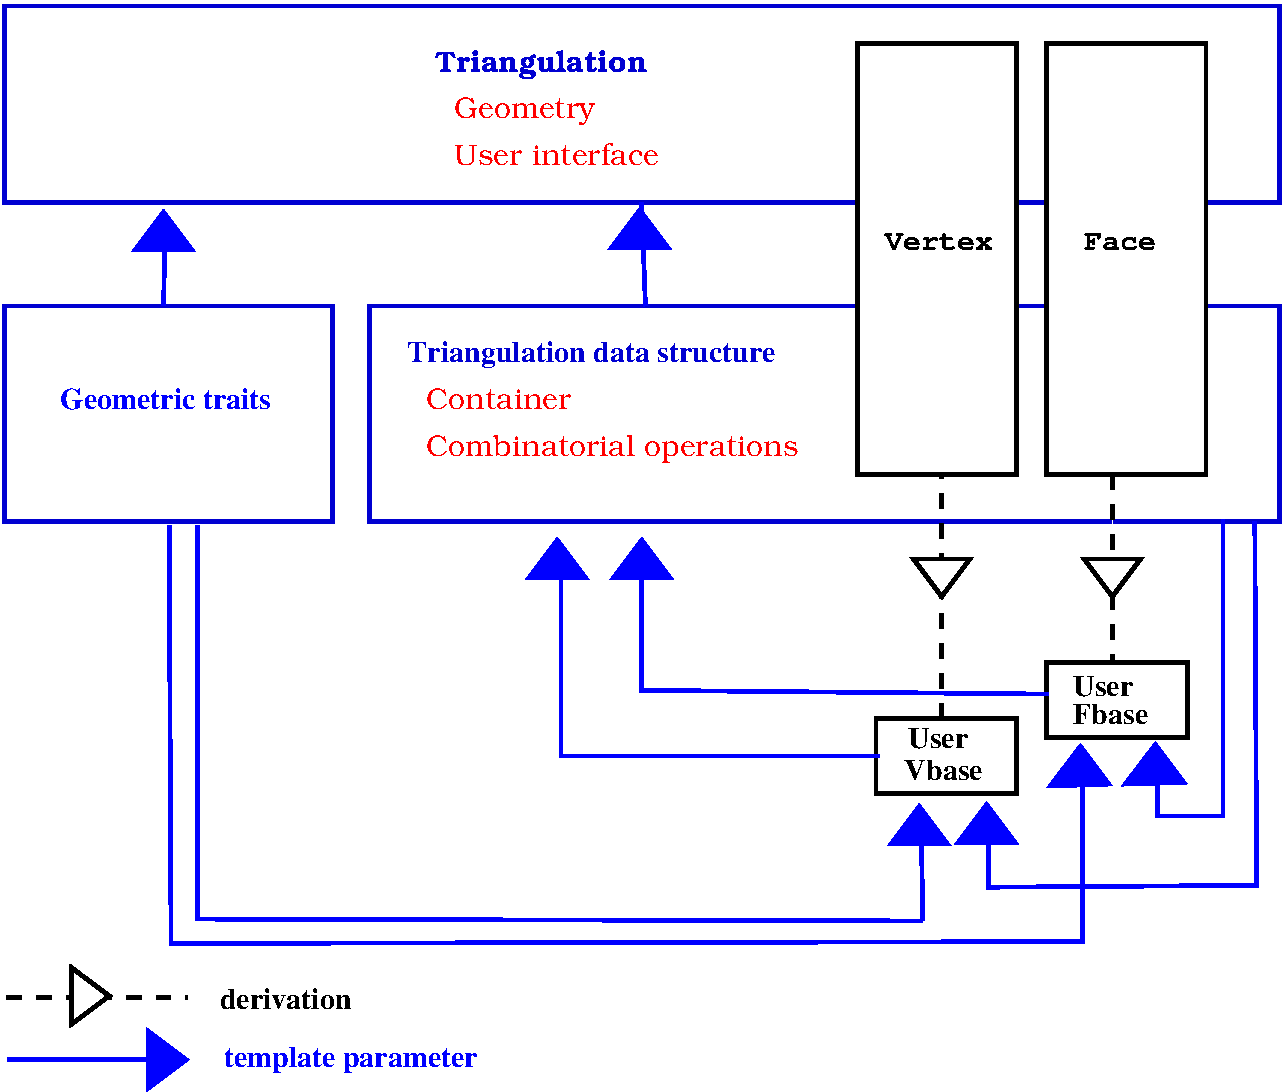
\includegraphics[width=13cm]{Triangulation_2/threelevels2}
\end{center}

\end{ccTexOnly}

\begin{ccHtmlOnly}
<CENTER>
<br>
<img border=0 src="./threelevels2.gif" align=center alt="Three_levels">
</CENTER>
\end{ccHtmlOnly}

\caption{The cyclic dependency in triangulations software design.
\label{2D_Triangulation_Fig_three_levels_2}}
\end{figure}

Previously, this cyclic dependency was avoided by 
using only \ccc{void*} pointers in the interface of base classes.
These \ccc{void*} were converted to appropriate types at the
triangulation data structure levels. This solution had some drawbacks
~: mainly the user could not add in the vertices or faces of the 
triangulation a functionality related to types defined by 
the triangulation data structure, for instance a handle to a vertex,
and he was lead to use himself 
\ccc{void*}  pointers).
The new solution to resolve the template dependency
is based on a rebind mechanism similar to the mechanism used in the 
standard allocator class std::allocator. The rebind mechanism
is described in Section~\ref{2D_TDS_default} 
of Chapter~\ref{Chapter_2D_Triangulation_Data_Structure}.
For now, we will just notice that the design
requires
the existence in the vertex and face base classes 
of a nested template class
\ccc{Rebind_TDS} defining a type \ccc{Other} used by
the rebinding mechanism.


The two following examples show how the user
can  put in use the flexibility offered by the
base classes parameters.

\subsection*{Adding colors} 

The first example corresponds to a case where the user wishes to add in 
the vertices or faces of the triangulation  an additional information
that does not depend on types provided
by the triangulation data structure. 
In that case, predefined classes
\ccc{Triangulation_vertex_base_with_info_2<Info,Traits,Vb>}
or \ccc{Triangulation_face_base_with_info_2<Info,Traits,Vb>}
can be used. Those classes have
a template parameter \ccc{Info} devoted to
handle additional information.
The following examples shows how to add a 
\ccc{CGAL::Color} in the triangulation faces.


\ccIncludeExampleCode{Triangulation_2/colored_face.C}

\subsection*{Adding handles}

The second example  shows how the user can  still
derive and plug in his own vertex 
or face class when he would like to have  
additional functionalities depending on types provided by the triangulation
data structure. 


\ccIncludeExampleCode{Triangulation_2/adding_handles.C}


\section{Design and Implementation History}

The code of this package is the result of a long development
process. Here follows a tentative list of people
who added their stone to this package~:
Jean-Daniel Boissonnat, Herv\'e Br\"onnimann, 
Olivier Devillers, Andreas Fabri, Fr\'ed\'eric Fichel,
Julia Fl\"ototto, Monique Teillaud and Mariette Yvinec.






